\chapter{Mean-Field Theory in Hubbard lattices}\label{appendix:mean-field-hubbard}

In this Appendix the Mean-Field solutions to the Hubbard hamiltonian,
\[
	\hat H = 
	-t \sum_{\langle ij \rangle} \sum_\sigma \hat c_{i\sigma}^\dagger \hat c_{j\sigma}
	+ U \sum_i \hat n_{i\uparrow} \hat n_{i\downarrow}
	\qquad
	t, U  > 0
\]
are described. The discussion is limited to the two-dimensional square lattice. The two-dimensional square lattice extension of the two-sites model can be studied by the means of Mean Field Theory. We have:
\[
\begin{aligned}
	\hat n_{i\uparrow} \hat n_{i\downarrow} &= \left( \ev{\hat n_{i\uparrow}} + \delta \hat n_{i\uparrow} \right) \left( \ev{\hat n_{i\downarrow}} + \delta \hat n_{i\downarrow} \right) \\
	&\simeq \ev{\hat n_{i\uparrow}} \ev{\hat n_{i\downarrow}} +  \delta \hat n_{i\uparrow} \ev{\hat n_{i\downarrow}} + \ev{\hat n_{i\uparrow}} \delta \hat n_{i\downarrow} + \mathcal{O} \left(\delta n^2\right) \\
	&= - \ev{\hat n_{i\uparrow}} \ev{\hat n_{i\downarrow}} + \hat n_{i\uparrow} \ev{\hat n_{i\downarrow}} + \ev{\hat n_{i\uparrow}} \hat n_{i\downarrow} + \mathcal{O} \left(\delta n^2\right)
\end{aligned}
\]
where $\delta \hat n_{i\sigma} \equiv \hat n_{i\sigma} - \ev{\hat n_{i\sigma}}$ and orders higher than first have been ignored, assuming negligible fluctuations around the equilibrium single-site population. The first term of the above three can be neglected at fixed particles number, being a pure energy shift. 

\section{Ferromagnetic solution}

The Mean-Field Theory ferromagnetic solution prescribes an uniformly magnetized lattice,
\[
	\ev{\hat n_{i\uparrow}} = n+m
	\qquad
	\ev{\hat n_{i\downarrow}} = n-m
\]
where $n$ is the site electron density and $m$ is the density unbalance, leading to a magnetization per site $2m$. The mean-field hamiltonian with these substitutions becomes:
\[
\begin{aligned}
	\hat H &\simeq 
	-t \sum_{\langle ij \rangle} \sum_\sigma \hat c_{i\sigma}^\dagger \hat c_{j\sigma}
	+ U \sum_i \left[
		\hat n_{i\uparrow} \ev{\hat n_{i\downarrow}} + \ev{\hat n_{i\uparrow}} \hat n_{i\downarrow} 
	\right] \\
	&= -t \sum_{\langle ij \rangle} \sum_\sigma \hat c_{i\sigma}^\dagger \hat c_{j\sigma}
	+ nU \sum_i \left[
		\hat n_{i\uparrow} + \hat n_{i\downarrow} 
	\right] - mU \sum_i \left[
		\hat n_{i\uparrow} - \hat n_{i\downarrow} 
	\right]
\end{aligned}
\]
Fourier transforming,
\[
\begin{aligned}
	-t \sum_{\langle ij \rangle} \sum_\sigma \hat c_{i\sigma}^\dagger \hat c_{j\sigma} &= -2t \sum_{\mathbf{k}\sigma} \left[
		\cos(k_x) + \cos(k_y)
	\right] \hat n_{\mathbf{k}\sigma} \\
	nU \sum_i \left[
		\hat n_{i\uparrow} + \hat n_{i\downarrow} 
	\right] &= nU \sum_{\mathbf{k}\sigma} \hat n_{\mathbf{k}\sigma} \\
	mU \sum_i \left[
		\hat n_{i\uparrow} - \hat n_{i\downarrow} 
	\right] &= mU \sum_{\mathbf{k}\sigma} \left[
		\hat n_{\mathbf{k}\uparrow} - \hat n_{\mathbf{k}\downarrow}
	\right]
\end{aligned}
\]
having used adimensional lattice momenta. For a square lattice, the Brillouin Zone is delimited by
\[
	\mathbf{k} \in [-\pi,\pi] \times [-\pi,\pi]
\]
The hopping single-state energy is given by
\[
	\epsilon_{\mathbf{k}}^{(0)} = -2t \left[
		\cos(k_x) + \cos(k_y)
	\right]
\]
represented as a band in Fig.~\ref{appfig:ferromagnetic-3d-band}. At $U=0$, the mean-field ferromagnetic state fills the band bottom-up. The single-state energy becomes:
\[
\begin{aligned}
	\epsilon_{\mathbf{k}\uparrow} &= U \left(
		n-m
	\right) - 2t \left[
		\cos(k_x) + \cos(k_y)
	\right] \\
	\epsilon_{\mathbf{k}\downarrow} &= U \left(
		n+m
	\right) - 2t \left[
		\cos(k_x) + \cos(k_y)
	\right]
\end{aligned}
\]
Now it is a matter of finding the optimal value for $m$, minimizing the total energy at fixed filling $\rho = 2n$. Notice that said minimization is performed parametrically varying the magnetization $m$, inside the ferromagnetic-polarized space. As it turns out, for strong local repulsion $U/t \gg 1$, antiferromagnetic ordering is preferred. Comparison is needed in order to assess which magnetic ordering is preferred.

Consider the half-filling situation. An unpolarized system will have $n=1/4$, $m=0$: this implies $\ev{\hat n_{i\uparrow}} = \ev{\hat n_{i\downarrow}} = 1/4$. A perfectly up-ferromagnetic system, $n=1/4$, $m=1/4$: then $\ev{\hat n_{i\uparrow}} = 1/2$ and $\ev{\hat n_{i\downarrow}} = 0$. \todo

\begin{figure}
	\centering
	\begin{tikzpicture}
	\begin{axis}[
			axis on top,
			axis lines=center,
			xmin=-1.3, xmax=1.3,
			ymin=-1.3, ymax=1.3,
			zmin=-2.5, zmax=2.5,
			xtick={-1,1},
			ytick={-1,1},
			ztick={-2,2},
			xticklabels={$-\pi$,$\pi$},
			yticklabels={$-\pi$,$\pi$},
			zticklabels={$-2t$,$2t$},
			xlabel={$k_x$},
			ylabel={$k_y$},
			zlabel={$\epsilon_{\mathbf{k}}^{(0)}$},
			xlabel style={anchor=west},
			ylabel style={anchor=south west},
			zlabel style={anchor=south},
			width=\textwidth,
			view/az=15,
			view/el=30,
		]
		\addplot3[
			domain=-1:0,
			color=tabred,
			dashed,
		]
		(
			{x},
			{-1-x},
			{0}
		);
		\addplot3[
			domain=0:1,
			color=tabred,
			dashed,
		]
		(
			{x},
			{-1+x},
			{0}
		);
		\addplot3[
			domain=-1:0,
			color=tabred,
			dashed,
		]
		(
			{x},
			{1+x},
			{0}
		);
		\addplot3[
			domain=0:1,
			color=tabred,
			dashed,
		]
		(
			{x},
			{1-x},
			{0}
		);
		
		\addplot3[
			domain=-1:1,
			samples=25,
			smooth,
			surf,
			opacity=0.2,
			colormap name=tab
		] { -cos(deg(pi*x))-cos(deg(pi*y)) };
	\end{axis}
\end{tikzpicture}
	\caption{Depiction of the Hubbard square lattice hopping band $\epsilon_{\mathbf{k}}^{(0)} = -2t[\cos(k_x) + \cos(k_y)]$. The red lines mark the zero-energy intersection.}
	\label{appfig:ferromagnetic-3d-band}
\end{figure}

\section{Antiferromagnetic solution}

Consider now an AF mean-field solution. Let me change notation for a brief moment, indicating each site as
\[
	i \to \mathbf{r} = (x,y)
	\qquad
	x,y \in \mathbb{N}
\]
The mean-field AF solution at half-filling is the uniform-modulated magnetization
\[
	m_\mathbf{r} = (-1)^{x+y} m
	\qquad
	m \in [-1,1]
\]
and a mean-field Ansatz
\begin{equation}\label{appeq:af-mean-field-ansatz}
	\ev{\hat n_{\mathbf{r}\uparrow}} = n+m_\mathbf{r}
	\qquad
	\ev{\hat n_{\mathbf{r}\downarrow}} = n-m_\mathbf{r}
\end{equation}
With respect to the solution presented above, the only detail changing is the last term,
\begin{equation}\label{appeq:hubbard-mean-field-hamiltonian}
	\hat H = -t \sum_{\langle \mathbf{r}\mathbf{r}' \rangle} \sum_\sigma \hat c_{\mathbf{r}\sigma}^\dagger \hat c_{\mathbf{r}'\sigma}
	+ nU \sum_\mathbf{r} \left[
		\hat n_{\mathbf{r}\uparrow} + \hat n_{\mathbf{r}\downarrow}
	\right] - mU \sum_\mathbf{r} (-1)^{x+y} \left[
		\hat n_{\mathbf{r}\uparrow} - \hat n_{\mathbf{r}\downarrow}
	\right]
\end{equation}
Fourier-transforming, the phase factor can be absorbed in the destruction operator inside of $\hat n_{\mathbf{r}\sigma}$:
\[
\begin{aligned}
	\sum_\mathbf{r} (-1)^{x+y} \hat n_{\mathbf{r}\sigma} &= \sum_\mathbf{r} (-1)^{x+y} \hat c_{\mathbf{r}\sigma}^\dagger \hat c_{\mathbf{r}\sigma} \\
	&= 
	\sum_\mathbf{r} e^{i \bm{\pi} \cdot \mathbf{r}}
	\frac{1}{L} \sum_{\mathbf{k} \in \mathrm{BZ}} e^{i \mathbf{k} \cdot \mathbf{r}} \hat c_{\mathbf{k}\sigma}^\dagger \frac{1}{L} \sum_{\mathbf{k}' \in \mathrm{BZ}} e^{-i \mathbf{k}' \cdot \mathbf{r}} \hat c_{\mathbf{k}'\sigma} \\
	&= \sum_{\mathbf{k} \in \mathrm{BZ}} \sum_{\mathbf{k}' \in \mathrm{BZ}} \hat c_{\mathbf{k}\sigma}^\dagger \hat c_{\mathbf{k}'\sigma} \frac{1}{L^2} \sum_\mathbf{r} e^{-i [\mathbf{k}' - (\mathbf{k} + \bm{\pi}) ] \cdot \mathbf{r}} \\
	&= \sum_{\mathbf{k} \in \mathrm{BZ}} \hat c_{\mathbf{k}\sigma}^\dagger \hat c_{\mathbf{k}+\bm{\pi}\sigma}
\end{aligned}
\]
where $\bm{\pi} = (\pi,\pi)$. It follows:
\[
mU \sum_\mathbf{r} (-1)^{x+y} \left[
		\hat n_{\mathbf{r}\uparrow} - \hat n_{\mathbf{r}\downarrow}
	\right] = \Delta \sum_{\mathbf{k} \in \mathrm{BZ}} \left[
		\hat c_{\mathbf{k}\uparrow}^\dagger \hat c_{\mathbf{k}+\bm{\pi}\uparrow} - \hat c_{\mathbf{k}\downarrow}^\dagger \hat c_{\mathbf{k}+\bm{\pi}\downarrow}
	\right]
	\qq{where}
	\Delta \equiv mU
\]

\begin{figure}
	\centering
	\subfloat[Alternative band.]{
		% It's easier to rotate coordinates and hide axis than
% define a tilted rectangular domain?

\begin{tikzpicture}
	\begin{axis}[
			axis on top,
			axis lines=none, % Support axis
			xmin=-1.3, xmax=1.3,
			ymin=-1.3, ymax=2.3,
			zmin=-2.5, zmax=2.5,
			view/az=65,
			view/el=30,
			width=0.7\textwidth
		]
		\addplot3[
			domain=-0.707:0.707,
			color=tabred,
		]
		(
			{x},
			{0.707},
			{0}
		);
		\addplot3[
			domain=-0.707:0.707,
			color=tabred,
		]
		(
			{x},
			{-0.707},
			{0}
		);
		\addplot3[
			domain y=-0.707:0.707,
			color=tabred,
		]
		(
			{0.707},
			{y},
			{0}
		);
		\addplot3[
			domain y=-0.707:0.707,
			color=tabred,
		]
		(
			{-0.707},
			{y},
			{0}
		);
		
		\draw[color=black, line width=0.2pt, -stealth]
			(0,0,0) -- (0.2,0.2,0) node[anchor=west, yshift=-0.2em]
				{\tiny $k_x$};
		\draw[color=black, line width=0.2pt, -stealth]
			(0,0,0) -- (-0.25,0.25,0) node[anchor=south, xshift=0.2em, yshift=-0.1em]
				{\tiny $k_y$};
		
		\node[color=tabred, anchor=south, yshift=0.2em]
			at (-0.707,0,0)
				{$\mathrm{MBZ}$};

		\draw[color=gray, -stealth]
			(0,0,0) -- (0,{sqrt(2)},0);

		\fill[color=tabred]
			(0,0,0) circle (1pt) node[anchor=east]
				{$\mathbf{0}$};
		
		\fill[color=tabblue]
			(0,{sqrt(2)},0) circle (1pt) node[anchor=west]
				{$\bm{\pi}$};
		
		\addplot3[
			domain=-0.707:0.707,
			y domain=-0.707:2.121,
			samples=25,
			smooth,
			surf,
			opacity=0.2,
			colormap name=tab
		] { -cos(deg(
				pi * (x-y)/sqrt(2)	% Rotated coordinates
			))-cos(deg(
				pi* (x+y)/sqrt(2)	% Rotated coordinates
			)) };
	\end{axis}
\end{tikzpicture}
		\label{appsubfig:alternative-ferromagnetic-3d-band}
	}
	\subfloat[Contour plot.]{
		\begin{tikzpicture}
	\begin{axis}[
			axis x line=center,
			axis y line=center,
			axis z line=none,
			xmin=-2.3, xmax=2.3,
			ymin=-2.3, ymax=2.3,
			zmin=-2.5, zmax=2.5,
			xtick={1},
			ytick={1},
			xticklabel={$\pi$},
			yticklabel={$\pi$},
			xlabel={$k_x$},
			ylabel={$k_y$},
			xlabel style={anchor=west},
			ylabel style={anchor=south},
			view/az=0,
			view/el=90,
			width=0.4\textwidth,
			height=0.4\textwidth
		]
		\addplot3[
			domain=-1:0,
			color=tabred,
			dashed,
		]
		(
			{x},
			{-1-x},
			{0}
		);
		\addplot3[
			domain=0:1,
			color=tabred,
			dashed,
		]
		(
			{x},
			{-1+x},
			{0}
		);
		\addplot3[
			domain=-1:0,
			color=tabred,
			dashed,
		]
		(
			{x},
			{1+x},
			{0}
		);
		\addplot3[
			domain=0:1,
			color=tabred,
			dashed,
		]
		(
			{x},
			{1-x},
			{0}
		);
		
		\addplot3[
			domain=-2:2,
			samples=25,
			smooth,
			contour filled={number=10},
			opacity=0.45,
		] { -cos(deg(pi*x))-cos(deg(pi*y)) };
		
		\node[color=tabred, anchor=south east, xshift=0.3em]
			at (-1,0,0)
				{\tiny $\mathrm{MBZ}$};
		
		\draw[color=gray, -stealth]
			(0,0,0) -- (1,1,0);
		
		\fill[color=tabred]
			(0,0,0) circle (0pt) node[anchor=south east]
				{$\mathbf{0}$};
		
		\fill[color=tabblue]
			(1,1,0) circle (1pt) node[anchor=west]
				{$\bm{\pi}$};
		
	\end{axis}

	% Fine tuned
	\fill[color=tabred]
		(2.21,2.21) circle (1pt);
	
\end{tikzpicture}
		\label{appsubfig:ferromagnetic-contour}
	}
	\caption{Alternative depiction of the Hubbard square lattice hopping band previously reported in Fig.~\ref{appfig:ferromagnetic-3d-band}. The Magnetic Brillouin Zone ($\mathrm{MBZ}$) is delimited by the zero-energy contour and is indicated in figure. As it is evident, energy sign flips by taking a $(\pi,\pi)$ translation in $\mathbf{k}$ space.}
	\label{appfig:alternative-ferromagnetic-band}
\end{figure}

Consider the band of Fig.~\ref{appfig:ferromagnetic-3d-band} at half-filling. As does \citeauthor{fabrizio2022course} \cite{fabrizio2022course}, the area delimited externally by the solid lines at zero energy is denominated ``Magnetic Brillouin Zone'' ($\mathrm{MBZ}$). The periodicity of $\mathbf{k}$ space guarantees that the full $\mathrm{BZ}$ can be taken as well to be the one of Fig.~\ref{appsubfig:alternative-ferromagnetic-3d-band}. Then:
\begin{align}
	\sum_{\mathbf{k} \in \mathrm{BZ}}
	\hat c_{\mathbf{k}\uparrow}^\dagger \hat c_{\mathbf{k}+\bm{\pi}\uparrow} &= \sum_{\mathbf{k} \in \mathrm{MBZ}}
	\left[
		\hat c_{\mathbf{k}\uparrow}^\dagger \hat c_{\mathbf{k}+\bm{\pi}\uparrow} + \hat c_{\mathbf{k}+\bm{\pi}\uparrow}^\dagger \hat c_{\mathbf{k}+2\bm{\pi}\uparrow}
	\right] \nonumber \\
	&= \sum_{\mathbf{k} \in \mathrm{MBZ}}
	\left[
		\hat c_{\mathbf{k}\uparrow}^\dagger \hat c_{\mathbf{k}+\bm{\pi}\uparrow} + \hat c_{\mathbf{k}+\bm{\pi}\uparrow}^\dagger \hat c_{\mathbf{k}\uparrow}
	\right] \label{appeq:mixed-cc-term-intermediate-passage}
\end{align}
and the same applies for spin $\downarrow$. Periodicity by shifts $2\bm{\pi}$ has been used. Now, define the Nambu spinors:
\[
	\hat \Psi_{\mathbf{k}\sigma} \equiv \begin{bmatrix}
		\hat c_{\mathbf{k}\sigma} \\
		\hat c_{\mathbf{k}+\bm{\pi}\sigma} 
	\end{bmatrix}
\]
and a spin-wise gap,
\[
	\Delta_\uparrow = \Delta
	\qquad
	\Delta_\downarrow = -\Delta
\]
At fixed filling, the $U$ term is a pure energy shift, thus will be neglected. The kinetic term transforms as
\[
\begin{aligned}
	-t \sum_{\langle ij \rangle} \sum_\sigma \hat c_{i\sigma}^\dagger \hat c_{j\sigma} &= \sum_{\mathbf{k} \in \mathrm{BZ}} \sum_\sigma \epsilon_\mathbf{k}^{(0)} \hat c_{\mathbf{k}\sigma}^\dagger \hat c_{\mathbf{k}\sigma} \\ 
	&= \sum_{\mathbf{k} \in \mathrm{MBZ}} \sum_\sigma \left[
		\epsilon_\mathbf{k}^{(0)} \hat c_{\mathbf{k}\sigma}^\dagger \hat c_{\mathbf{k}\sigma}
		+ \epsilon_{\mathbf{k}+\bm{\pi}}^{(0)} \hat c_{\mathbf{k}+\bm{\pi}\sigma}^\dagger \hat c_{\mathbf{k}+\bm{\pi}\sigma}
	\right] \\
	&= \sum_{\mathbf{k} \in \mathrm{MBZ}} \sum_\sigma \epsilon_{\mathbf{k}}^{(0)}  \left[
		\hat c_{\mathbf{k}\sigma}^\dagger \hat c_{\mathbf{k}\sigma}
		- \hat c_{\mathbf{k}+\bm{\pi}\sigma}^\dagger \hat c_{\mathbf{k}+\bm{\pi}\sigma}
	\right] \\ 
\end{aligned}
\]
In the second passage, the sum over the full $\mathrm{BZ}$ was written considering that the entirety of the zone is given by all the points in the $\mathrm{MBZ}$ plus their conjugates obtained by a $\bm{\pi}$ shift in the flipped band. As depicted in Fig.~\ref{appsubfig:alternative-ferromagnetic-3d-band}, kinetic energy is anti-periodic in $\mathbf{k}$ space by a vector $\bm{\pi}$. This anti-periodicity accounts for the minus sign arising in the third passage. The hamiltonian is then given by:
\begin{equation}\label{appeq:hubbard-bogoliubov-hamiltonian}
	\hat H = \sum_{\mathbf{k} \in \mathrm{MBZ}} \sum_\sigma \hat \Psi_{\mathbf{k}\sigma}^\dagger h_{\mathbf{k}\sigma} \hat \Psi_{\mathbf{k}\sigma}
	\qq{being}
	h_{\mathbf{k}\sigma} \equiv \begin{bmatrix}
		\epsilon_\mathbf{k}^{(0)} & -\Delta_\sigma \\
		-\Delta_\sigma & - \epsilon_\mathbf{k}^{(0)}
	\end{bmatrix}
\end{equation}
Notice: the Nambu hamiltonian is a $2\times2$ matrix over the $\mathrm{MBZ}$ -- which is half the full $\mathrm{BZ}$, coherently with a solution which essentially bipartites the lattice giving back a double sized unit cell.

\begin{figure}
	\centering
	\def\DeltaParameter{0.6}
\def\XiParameter{0.4} % Here $\epsilon$, import
\begin{tikzpicture}
	\begin{axis}[
			axis x line=center,
			axis y line=center,
			axis z line=center,
			axis on top,
			xlabel={$x$},
			ylabel={$y$},
			zlabel={$z$},
			xlabel style={right},
			ylabel style={above left, yshift=-0.4em},
			zlabel style={above},
			xtick={-\DeltaParameter,\DeltaParameter},
			ytick=\empty,
			ztick={-\XiParameter,\XiParameter},
			xticklabels={$-\Delta$,$\Delta$},
			yticklabel=\empty,
			zticklabels={$-\epsilon_\mathbf{k}^{(0)}$,$\epsilon_\mathbf{k}^{(0)}$},
			xticklabel style=below,
			yticklabel style=\empty,
			zticklabel style=left,
			xmin=-1, xmax=1,
			ymin=-0.25, ymax=0.25,
			zmin=-1, zmax=1,
			view/h=-30,
			view/v=15,
			scale=1.5,
		]
		
		% Dashed lines
		\draw[color=gray!70,dashed]
			(axis cs:\DeltaParameter,0,0) -- (axis cs:\DeltaParameter,0,\XiParameter);
		\draw[color=gray!70,dashed]
			(axis cs:0,0,\XiParameter) -- (axis cs:\DeltaParameter,0,\XiParameter);
		\draw[color=gray!70,dashed]
			(axis cs:-\DeltaParameter,0,0) -- (axis cs:-\DeltaParameter,0,-\XiParameter);
		\draw[color=gray!70,dashed]
			(axis cs:0,0,-\XiParameter) -- (axis cs:-\DeltaParameter,0,-\XiParameter);
		
		% Eigenstates
		\filldraw[color=tabblue] 
			(axis cs:\DeltaParameter,0,\XiParameter) circle (1.2pt) node[anchor=south west]
				{$E_\mathbf{k}$};
		\filldraw[color=tabred] 
			(axis cs:-\DeltaParameter,0,-\XiParameter) circle (1.2pt) node[anchor=north east]
				{$-E_\mathbf{k}$};
		
		% Pseudo field
		\draw[color=tabgreen,-stealth]
			(axis cs:0,0,0) -- (axis cs:\DeltaParameter,0,\XiParameter) node[anchor=north west,midway]
				{$\mathbf{b}_{\mathbf{k}\uparrow}$};
		
		% Angle
		\begin{scope}[canvas is zx plane at y=0]
			\draw[color=tabgreen] 
			(\XiParameter/2,0) arc [start angle=0,end angle=atan(\DeltaParameter/\XiParameter),radius=\XiParameter/2]
				node[anchor=south, xshift=0.2em, midway]
					{$2\theta_\mathbf{k}$};
		\end{scope}
		
	\end{axis}
\end{tikzpicture}
	\caption{Pseudo-magnetic field originating from mean-field treatment of the square Hubbard hamiltonian. Here, only the $\sigma=\uparrow$}
	\label{appfig:pseudo-magnetic-field}
\end{figure}

The system ground-state is obtained by the means of a Bogoliubov rotation. The hamiltonian maps onto the simple one of a spin in a magnetic field,
\[
	h_{\mathbf{k}\sigma} = \epsilon_\mathbf{k}^{(0)} \tau^z - \Delta_\sigma \tau^x
\]
being $\tau^\alpha$ the Pauli matrices. Then, defining
\[
	\hat s_{\mathbf{k}\sigma}^\alpha \equiv \hat \Psi_{\mathbf{k}\sigma}^\dagger \tau^\alpha \hat \Psi_{\mathbf{k}\sigma}
	\qq{and}
	\mathbf{b}_{\mathbf{k}\sigma} \equiv \begin{bmatrix}
		-\Delta_\sigma \\ 0 \\ \epsilon_\mathbf{k}^{(0)} 
	\end{bmatrix}
\]
one gets:
\begin{equation}\label{appeq:hubbard-bogoliubov-hamiltonian-pseudofields}
	\hat H = \sum_{\mathbf{k} \in \mathrm{MBZ}} \sum_\sigma \mathbf{b}_{\mathbf{k}\sigma} \cdot \hat{\mathbf{s}}_{\mathbf{k}\sigma}
	\qq{where}
	\hat{\mathbf{s}}_{\mathbf{k}\sigma} = \begin{bmatrix}
		\hat s_{\mathbf{k}\sigma}^x \\
		\hat s_{\mathbf{k}\sigma}^y \\
		\hat s_{\mathbf{k}\sigma}^z
	\end{bmatrix}
\end{equation}
The hamiltonian represents a system of spins subject to local magnetic fields, each tilted by an angle $\tan(2\theta_{\mathbf{k}\sigma}) = \Delta_\sigma/\epsilon_{\mathbf{k}}^{(0)}$, as sketched in Fig.~\ref{appfig:pseudo-magnetic-field}. At any finite temperature, the ground-state of such a system is well-known. Diagonalization of each $h_{\mathbf{k}\sigma}$ is obtained trivially by a simple rotation around the $y$ axis:
\[
	d_{\mathbf{k}\sigma} = W_{\mathbf{k}\sigma} h_{\mathbf{k}\sigma} W_{\mathbf{k}\sigma}^\dagger
\]
where
\[
	d_{\mathbf{k}\sigma} = \begin{bmatrix}
		- E_\mathbf{k} & \\
		& E_\mathbf{k}
	\end{bmatrix}
	\qq{and}
	W_{\mathbf{k}\sigma} = \exp{i \frac{2\theta_{\mathbf{k}\sigma} - \pi}{2}
	\tau^y}
\]
Note that rotation is taken to be of an angle $2\theta_{\mathbf{k}\sigma} - \pi$ in order to anti-align the pseudo-spin with the magnetic field of Fig.~\ref{appfig:pseudo-magnetic-field} and thus order the eigenvalues as in $d_{\mathbf{k}\sigma}$, with the smaller one in the top-left corner of the matrix and the larger one in the bottom-right corner. The explicit form of the transformation matrix is thus
\begin{equation}\label{appeq:W-explicit-form}
	W_{\mathbf{k}\sigma} = \begin{bmatrix}
		\cos \theta_{\mathbf{k}\sigma} & - \sin \theta_{\mathbf{k}\sigma} \\
		\sin \theta_{\mathbf{k}\sigma} & \cos \theta_{\mathbf{k}\sigma}
	\end{bmatrix} \begin{bmatrix}
		& -1 \\
		1 &
	\end{bmatrix} = \begin{bmatrix}
		- \sin \theta_{\mathbf{k}\sigma} & - \cos \theta_{\mathbf{k}\sigma} \\ 
		\cos \theta_{\mathbf{k}\sigma} & - \sin \theta_{\mathbf{k}\sigma}
	\end{bmatrix}
\end{equation}
Eigenvalues are:
\[
	E_\mathbf{k} \equiv \sqrt{\epsilon_{\mathbf{k}}^2 + \abs{\Delta_\sigma}^2}
\]
(superscript ``$(0)$'' has been dropped momentarily). Notice that the presence of an absolute value makes the eigenvalues independent of the $\sigma$ index. Eigenvector fermion operators are obtained simply as:
\begin{equation}\label{appeq:af-diagonalized-nambu-spinor}
	\hat\Gamma_{\mathbf{k}\sigma} = W_{\mathbf{k}\sigma} \hat \Psi_{\mathbf{k}\sigma}
\end{equation}
The $\hat\Gamma$ spinor operators are effectively free fermionic spinor fields and as such must be treated. Note that:
\begin{align}
	N &= \sum_{\mathbf{k}\sigma} \ev{\hat n_{\mathbf{k}\sigma}} \nonumber \\
	&= \sum_\sigma \sum_{\mathbf{k} \in \mathrm{MBZ}} \left\langle
		\hat n_{\mathbf{k}\sigma} + \hat n_{\mathbf{k}+\bm{\pi}\sigma}
	\right\rangle \nonumber \\
	&= \sum_\sigma \sum_{\mathbf{k} \in \mathrm{MBZ}} \left\langle
		\hat\Gamma_{\mathbf{k}\sigma}^\dagger
		\hat\Gamma_{\mathbf{k}\sigma}
	\right\rangle \nonumber \\
	&= 2 \sum_{\mathbf{k} \in \mathrm{MBZ}} \left[
		f\left(-E_\mathbf{k}; \beta,\mu \right) + f \left( E_\mathbf{k}; \beta,\mu \right)
	\right] \label{appeq:spinor-particle-number-formula}
\end{align}
being $f$ be the Fermi-Dirac distribution at inverse temperature $\beta$ and chemical potential $\mu$,
\[
	f(\epsilon;\beta,\mu) = \frac{1}{e^{\beta(\epsilon-\mu)}+1} 
\]
The $2$ prefactor appeared because of spin degeneracy. Since the gapped bands refer to the smaller MBZ, thus exhibit the periodicity
\[
	E_\mathbf{k} = E_{\mathbf{k}+\bm{\pi}}
\]
it holds equivalently
\begin{equation}\label{appeq:spinor-particle-number-formula-BZ}
	N = \sum_{\mathbf{k} \in \mathrm{BZ}} \left[
		f\left(
			-E_\mathbf{k}; \beta,\mu 
		\right) + f \left(
			E_\mathbf{k}; \beta,\mu 
		\right)
	\right]
\end{equation}
as is obvious. The $2$ prefactor was absorbed in doubling the integration region, $\mathrm{MBZ}\to\mathrm{BZ}$. Next sections are devoted to simplify the above theoretical results in order to obtain an algorithmic estimation for the magnetization $m$, which is just the AF instability order parameter. 

\subsection{Theoretical mean-field solution}

A convergence algorithm can be designed to find the Hartree-Fock solution to the model. Ultimately, we aim to extract $m$ self-consistently. Since
\[
\begin{aligned}
	m &= \frac{1}{2L^2} \sum_\mathbf{r} (-1)^{x+y} \left\langle
		\hat n_{\mathbf{r}\uparrow} - \hat n_{\mathbf{r}\downarrow}
	\right\rangle \\
	&= \frac{1}{2L^2} \sum_{\mathbf{k} \in \mathrm{BZ}} \left\langle
		\hat c_{\mathbf{k}\uparrow}^\dagger \hat c_{\mathbf{k}+\bm{\pi}\uparrow} - \hat c_{\mathbf{k}\downarrow}^\dagger \hat c_{\mathbf{k}+\bm{\pi}\downarrow}
	\right\rangle \\
	&= \frac{1}{2L^2} \sum_{\mathbf{k} \in \mathrm{MBZ}} \left\langle
			\left(
				\hat c_{\mathbf{k}\uparrow}^\dagger \hat c_{\mathbf{k}+\bm{\pi}\uparrow} + \hat c_{\mathbf{k}+\bm{\pi}\uparrow}^\dagger \hat c_{\mathbf{k}\uparrow}	
			\right) - \left(
				\hat c_{\mathbf{k}\downarrow}^\dagger \hat c_{\mathbf{k}+\bm{\pi}\downarrow} + \hat c_{\mathbf{k}+\bm{\pi}\downarrow}^\dagger \hat c_{\mathbf{k}\downarrow}	
			\right)
		\right\rangle
\end{aligned}
\]
In the last passage, Eq.~\eqref{appeq:mixed-cc-term-intermediate-passage} has been used. Then magnetization can be computed simply as
\begin{equation}\label{appeq:antiferromagnet-magnetization-self-consistence-abstract}
	m = \frac{1}{2L^2} \sum_{\mathbf{k} \in \mathrm{MBZ}} \left[
		\left\langle 
			\hat \Psi_{\mathbf{k}\uparrow}^\dagger \tau^x \hat \Psi_{\mathbf{k}\uparrow}
		\right\rangle - \left\langle 
			\hat \Psi_{\mathbf{k}\downarrow}^\dagger \tau^x \hat \Psi_{\mathbf{k}\downarrow}
		\right\rangle
	\right]
\end{equation}
In this equation, spin expectation values appear:
\[
	\left\langle 
		\hat \Psi_{\mathbf{k}\sigma}^\dagger \tau^x \hat \Psi_{\mathbf{k}\sigma}
	\right\rangle = \ev{\hat s_{\mathbf{k}\sigma}^x}
\]
Now discussion is divided in two parts: zero temperature and finite temperature.

\subsubsection{Zero temperature solution}

For a spin system at zero temperature, the spin operator expectation value anti-aligns with the external field,
\[
	\ev{\hat s_{\mathbf{k}\sigma}^x} = \sin(2\theta_{\mathbf{k}\sigma})
\]
(see Fig.~\ref{appfig:pseudo-magnetic-field}). Now, since $\Delta_\downarrow = - \Delta_\uparrow$, it follows
\[
	\theta_{\mathbf{k}\uparrow} = -\theta_{\mathbf{k}\downarrow} \equiv \theta_\mathbf{k}
\]
Then, from Eq.~\eqref{appeq:antiferromagnet-magnetization-self-consistence-abstract}
\[
\begin{aligned}
	m &= \frac{1}{L^2} \sum_{\mathbf{k} \in \mathrm{MBZ}} \sin(2\theta_\mathbf{k}) \\
	&= \frac{1}{2L^2} \sum_{\mathbf{k} \in \mathrm{BZ}} \sin(2\theta_\mathbf{k})
\end{aligned}
\]
The last passage is due to the fact that the sum over the $\mathrm{MBZ}$ can be performed identically over $\mathrm{BZ}\setminus\mathrm{MBZ}$ and yield the same result. This is because of the lattice periodicity in reciprocal space. Then, finally:
\begin{equation}\label{appeq:antiferromagnet-magnetization-self-consistence-zero-temperature}
	m = \frac{1}{L^2} \sum_{\mathbf{k} \in \mathrm{BZ}} [ W_{\mathbf{k}\uparrow} ]_{11} [ W_{\mathbf{k}\uparrow}^\dagger ]_{21}
\end{equation}
where $\sin(2\theta_\mathbf{k}) = 2 \sin\theta_\mathbf{k} \cos\theta_\mathbf{k}$ has been used. As will become clear in next section, the sudden appearance of matrix elements of $W$ is not casual.

\subsubsection{Finite temperature solution}

At finite temperature $\beta$, discussion is analogous to the section above. Here will be treated somewhat more theoretically. Define the generic order parameter:
\[
	\Delta_{ij} (\mathbf{k}\sigma) \equiv \left\langle
		[
			\hat \Psi_{\mathbf{k}\sigma}^\dagger
		]_i [
			\hat \Psi_{\mathbf{k}\sigma}
		]_j
	\right\rangle
\]
In last section, the relevant indices $(i,j)$ were $(1,2)$ and $(2,1)$. Transform this order parameter,
\begin{align}
	\Delta_{ij} (\mathbf{k}\sigma) &= \sum_{i'j'} \left\langle
		[
			\hat\Gamma_{\mathbf{k}\sigma}^\dagger
		]_{i'} 
		[
			W_{\mathbf{k}\sigma}
		]_{i'i} [
			W_{\mathbf{k}\sigma}^\dagger
		]_{jj'}
		[
			\hat\Gamma_{\mathbf{k}\sigma}
		]_{j'}
	\right\rangle \nonumber \\
	&= 
	\sum_{i'j'} [
		W_{\mathbf{k}\sigma}
	]_{i'i} [
		W_{\mathbf{k}\sigma}^\dagger
	]_{jj'}
	\left\langle
		[
			\hat\Gamma_{\mathbf{k}\sigma}^\dagger
		]_{i'} 
		[
			\hat\Gamma_{\mathbf{k}\sigma}
		]_{j'}
	\right\rangle \nonumber \\
	&= 
	\sum_{i'j'} [
		W_{\mathbf{k}\sigma}
	]_{i'i} [
		W_{\mathbf{k}\sigma}^\dagger
	]_{jj'}
	\delta_{i'j'} f\left(
		[d_{\mathbf{k}\sigma}]_{i'i'}; \beta,\mu
	\right) \nonumber \\
	&= 
	\sum_{\ell=1}^2 [
		W_{\mathbf{k}\sigma}
	]_{\ell i} [
		W_{\mathbf{k}\sigma}^\dagger
	]_{j\ell}
	f\left(
		(-1)^\ell E_{\mathbf{k}\sigma}; \beta,\mu
	\right) \nonumber \\
	&= 
	[
		W_{\mathbf{k}\sigma}
	]_{1 i} [
		W_{\mathbf{k}\sigma}^\dagger
	]_{j 1} f\left(
		-E_\mathbf{k}; \beta,\mu
	\right) + [
		W_{\mathbf{k}\sigma}
	]_{2 i} [
		W_{\mathbf{k}\sigma}^\dagger
	]_{j 2} f\left(
		E_\mathbf{k}; \beta,\mu
	\right) \label{appeq:finite-temperature-order-parameter-derivation-intermediate}
\end{align}
In the second passage this distribution appeared because an expectation value over a gas of free $\Phi$ fermions was taken. Such an expectation value admits no off-diagonal values, hence the $\delta_{i'j'}$. The diagonal entries are precisely the definition of the Fermi-Dirac distribution for the given energy. At zero temperature and half-filling, the lower band $-E_\mathbf{k}$ is completely filled while the upper band $E_\mathbf{k}$ is empty. Substituting $f=1$ in the first term of line \eqref{appeq:finite-temperature-order-parameter-derivation-intermediate}, $f=0$ in the second and summing $\Delta_{12}$ and $\Delta_{21}$ as done in Eq.~\eqref{appeq:antiferromagnet-magnetization-self-consistence-abstract}, it's easy to derive the result of Eq.~\eqref{appeq:antiferromagnet-magnetization-self-consistence-zero-temperature}. At finite temperature, following the lead of the above paragraph, the antiferromagnetic instability order parameter $m$ will be given simply by
\begin{equation}\label{appeq:antiferromagnet-magnetization-self-consistence-finite-temperature}
	m = \frac{1}{2L^2} \sum_{\mathbf{k} \in \mathrm{BZ}} \sum_{\ell=1}^2 
	[
		W_{\mathbf{k}\uparrow}
	]_{\ell 1} [
		W_{\mathbf{k}\uparrow}^\dagger
	]_{2 \ell}
	f\left(
		(-1)^\ell E_\mathbf{k}; \beta,\mu
	\right)
\end{equation}
Then: mean-field approximations yield an estimate for the magnetization at a given temperature and chemical potential just by carefully combining the elements of the diagonalizing matrix $W$ of each Bogoliubov matrix $h_{\mathbf{k}\sigma}$.

\subsection{Hartree-Fock algorithm in reciprocal space}\label{appsubsec:hartree-fock-algorithm}

The above sections offers a self-consistency equation for the magnetization $m$; $W$ is determined by $m$ indeed. Then a self-consistent algorithm to search for a self consistent estimate for $m$ may be sketched:
\begin{enumerate}
	\setcounter{enumi}{-1}
	\item Algorithm setup: initialize a counter $i=1$ and choose:
	\begin{itemize}
		\item the local repulsion $U/t$ or equivalently the hopping amplitude $t/U$;
		\item the coarse-graining of the $\mathrm{BZ}$, which is, fix $L_x$ and $L_y$. Then 
		\[ 
			k_x = 2\pi n_x/L_x
			\qquad
			k_y = 2\pi n_y/L_y 
		\]
		where $-L_j/2 \le n_j \le L_j/2$, $n_j \in \mathbb{Z}$;
		\item the density $n$ or equivalently the doping $\delta \equiv n-0.5$;
		\item the inverse temperature $\beta$;
		\item the number of iterations $p \in \mathbb{N}$; 
		\item the mixing parameter $g \in [0,1]$;
		\item the tolerance parameters $\Delta_m, \Delta_n \in \mathbb{R}$ (respectively for magnetization and density);
	\end{itemize}
	\item {\color{tabred}
		Select a random starting value $m_0 \in [-(1-n),1-n]$
	};
	\item For each slot of the $\mathrm{BZ}$, initialize the appropriate $2\times2$ matrix $h_{\mathbf{k}\uparrow}$ as in Eq.~\eqref{appeq:hubbard-bogoliubov-hamiltonian};
	\item For the given hamiltonian, find the optimal chemical potential $\mu$ as follows:
	\begin{enumerate}
		\item Diagonalize $h_{\mathbf{k}\uparrow}[m_0, U]$ and obtain its eigenvalues $\pm E_\mathbf{k}[m_0, U$]; 
		\item Define the function of the chemical potential $\mu$,
		\[
			\delta n(\mu; \beta, m_0, U) \equiv 2 \left[
			f\left(-E_\mathbf{k}[U,m_0]; \beta,\mu \right) + f \left( E_\mathbf{k}[U,m_0]; \beta,\mu \right)
			\right] - n
		\]
		\item Find the root of $\delta n$, 
		\[
			\delta n(\mu_0) = 0
		\]
		Then $\mu_0$ is the chemical potential which, at magnetization $m_0$, realizes the best approximation of density $n$;
	\end{enumerate}
	\item {\color{tabred}
		Diagonalize the matrix $h_{\mathbf{k}\uparrow}$ and obtain $d_{\mathbf{k}\uparrow}$
	};
	\item Compute $m$ using Eq.~\eqref{appeq:antiferromagnet-magnetization-self-consistence-finite-temperature} with chemical potential $\mu_0$ and update the counter, $i \to i+1$;
	\item Check if $\abs{m-m_0} \le \delta_m$:
	\begin{itemize}
		\item If yes, halt;
		\item If not: check if $i > p$
		\begin{itemize}
			\item If yes, halt and consider choosing better tolerance and model parameters;
			\item If not, define 
			\[
				m_0 = gm + (1-g)m_0
			\]
			(logical assignment notation used) and repeat from step 2.
		\end{itemize}
	\end{itemize}
\end{enumerate}
In next section some results are briefly shown.

\subsubsection{Results}

\begin{figure}
	\centering
	\subfloat[Local repulsion $U/t$ depencence.]{
		\includegraphics[width=0.45\textwidth]{../Project/HartreeFock/analysis/Phase=AF/Scan/Setup=Test256/PlotOrderParameter/xVar=U/pVar=δ/m_t=1.0_V=0.0_Lx=256.0_β=Inf.pdf}
		\label{appsubfig:mU-beta=Inf}
	}
	\subfloat[Doping $\delta = n-0.5$ dependence.]{
		\includegraphics[width=0.45\textwidth]{../Project/HartreeFock/analysis/Phase=AF/Scan/Setup=Test256/PlotOrderParameter/xVar=δ/pVar=U/m_t=1.0_V=0.0_Lx=256.0_β=Inf.pdf}
		\label{appsubfig:dU-beta=Inf}
	}	
	\caption{Plots of the zero-temperature AF instability order parameter $m$ as a function of both the local repulsion $U/t$ (Fig.~\ref{appsubfig:mU-beta=Inf}) and the doping $\delta = n-1/2$ (Fig.~\ref{appsubfig:dU-beta=Inf}).}
	\label{appfig:mdU-beta=Inf}
\end{figure}

The algorithm sketched in the above paragraph was ran with the following setup:
\begin{lstlisting}[language=julia]
UU = [U for U in 0.5:0.5:10.0]      # Local repulsions
LL = [2^x for x in 5:7]             # Lattice sizes
dd = [d for d in 0.0:0.05:0.5]      # Dopings
bb = [0.1, 1.0, 10.0, 50.0, Inf]    # Inverse temperatures
p = 100                             # Max number of iterations
dm = 1e-4                           # Tolerance on magnetization
dn = 1e-2                           # Tolerance on density
g = 0.5                             # Mixing parameter
\end{lstlisting}
In Fig.~\ref{appfig:mdU-beta=Inf} plots at $\beta=\infty$ of the magnetization $m$ are reported. As is evident in Fig.~\ref{appsubfig:mU-beta=Inf}, disrupts AF ordering; the horizontal asymptote lowers as $\delta$ gets bigger, a mere consequence of the fact that the free space at each single-particle state in $k$-space shrinks as density increases; also, for $\delta > 0$, a finite magnetization $m$ exists only for $U \ge U_c[\delta]$ (a critical value parametrically dependent on doping). Fig.~\ref{appsubfig:dU-beta=Inf} shows the dependence of magnetization on doping at various fixed local repulsions $U$: once again, to dope the material disrupt AF ordering. Identical analysis have been performed for finite temperatures, leading to analogous results as long as $\beta \gtrsim 10$ and to $m \simeq 0$ for higher temperatures (predictably).

\subsection{An alternative (less efficient) real-space approach}

The theoretical derivation of the above paragraphs offers a simple description of the system anti-ferromagnetic instability as the instauration of a ground-state of quasiparticles. Here a self-consistent algorithmic extraction of the expected magnetization is presented, following \cite{scholle2023comprehensive}. Note that this algorithm is by far the least efficient, being performed in real space with dimensional exponential scaling in terms of computational time. It is here presented just for completeness as an alternative derivation. This algorithm can become useful for simulations not preserving space-translational invariance, e.g. introducing some degree of disorder. Consider a square lattice of $L_x \times L_y$ sites: the hamiltonian will be a matrix of dimension $2L_x L_y \times 2L_x L_y$,
\[
	[ \hat H ]_{(\mathbf{r}\sigma)(\mathbf{r}'\sigma')} = \mel{\Omega}{ \hat c_{\mathbf{r}\sigma} \hat H \hat c_{\mathbf{r}'\sigma'}^\dagger}{\Omega}
\]
For simplicity, in the following $D \equiv 2L_x L_y$. In this context, the following convention is used: the rows/column index entry $\alpha=(\mathbf{r}\sigma)$ is associated to a specific site $\mathbf{r}=(x,y)$ and spin $\sigma$ through the relation
\[
	\alpha = 2j_\mathbf{r}-\delta_{\sigma=\uparrow}
	\qq{where}
	j_\mathbf{r} = x+(y-1)L_x 
\]
Let me break this through. For each site $\mathbf{r}$, two sequential indices are provided ($2j_\mathbf{r}-1$, hosting spin $\uparrow$, and $2j_\mathbf{r}$, hosting spin $\downarrow$). $j_\mathbf{r}$ just orders the site rows-wise. This way, $(x,1)$ is assigned to $j_{(x,1)}=x$, while its NN one site above $(x,2)$ is assigned to an entry shifted by $L_x$, $j_{(x,2)}=x+L_x$. This is just a way of counting the site of a finite square lattice by sweeping along a row and then moving to the row above. Fig.~\ref{appfig:square-lattice-ordering} reports a scheme of the used site ordering.

\begin{figure}
	\centering
	\newcount\xLength
\xLength=4	% Even!
\newcount\yLength
\yLength=2	% Even!

\newcount\xStop
\xStop=\xLength
\divide\xStop by 2 \advance\xStop by -1\relax

\newcount\yStop
\yStop=\yLength
\divide\yStop by 2 \advance\yStop by -1\relax

\def\angle{60}
\def\arrowLength{0.5}

\def\scale{2}
\def\pointWidth{1.5/\scale}
% For now I leave here unchanged, but I would
% like to make the dimension of the points 
% independent of the scale. Which is, use 
% \pointWidth instead of a specific width in the 
% points definition.

\begin{tikzpicture}[scale=\scale]
	\draw[
		color=lightgray, dashed
	] 
		(0,0) grid ({\xLength+0.125}, {\yLength+0.125});
	
	% Nested, no indentation
	\foreach \x in {
		0,...,\xStop
	}{
		\foreach \y in {
			0,...,\yStop
		}{
			% Up sites
			\fill[color=tabred] 
				({2*\x},{2*\y}) circle (0.75pt)
				({2*\x+1},{2*\y+1}) circle (0.75pt)
			;
			
			% Down sites
			\fill[color=tabblue] 
				({2*\x},{2*\y+1}) circle (0.75pt)
				({2*\x+1},{2*\y}) circle (0.75pt)
			;
			
		}
	}
	
	% Border
	\foreach \x in {
		0, ..., \xStop
	}{
		\foreach \y in {
			0, ..., \yStop
		}{
			
			% Up sites
			\fill[color=tabred] 
				({2*\x},\yLength) circle (0.75pt)
				(\xLength,{2*\y}) circle (0.75pt)
			;
			
			% Down sites
			\fill[color=tabblue] 
				({2*\x+1},\yLength) circle (0.75pt)
				(\xLength,{2*\y+1}) circle (0.75pt)
			;
			
	}}
	
	% Topright
	\fill[color=tabred] 
		(\xLength,\yLength) circle (0.75pt);
	
	% Red labels
	\node[color=tabred, anchor=south west, align=center] 
		at (0,0)
			{\small $1 (\uparrow)$ \\ \small $2 (\downarrow)$};
	\node[color=tabred, anchor=south west, align=center] 
		at (2,0)
			{\small $5 (\uparrow)$ \\ \small $6 (\downarrow)$};
	\node[color=tabred, anchor=south west, align=center] 
		at (1,1)
			{\small $L_x+3 (\uparrow)$ \\ \small $L_x+4 (\downarrow)$};
	
	% Red labels
	\node[color=tabblue, anchor=south west, align=center] 
		at (1,0)
			{\small $3 (\uparrow)$ \\ \small $4 (\downarrow)$};
	\node[color=tabblue, anchor=south west, align=center] 
		at (0,1)
			{\small $L_x+1 (\uparrow)$ \\ \small $L_x+2 (\downarrow)$};
	\node[color=tabblue, anchor=south west, align=center] 
		at (2,1)
			{\small $L_x+5 (\uparrow)$ \\ \small $L_x+6 (\downarrow)$};
	
	
\end{tikzpicture}
	\caption{Schematics of the site ordering on a square lattice performed by sweeping along rows. Left-bottom side is one corner of the lattice. Red sites are characterized by $x+y$ being odd, blue sites by being even. The number reported near to each site is the $\alpha$ entry in the matrix representation for a finite square lattice.}
	\label{appfig:square-lattice-ordering}
\end{figure}

Within this convention, matrix elements $H_{\alpha\beta}$ are defined by:
\begin{itemize}
	\item If $\sigma=\sigma'$ and $\mathbf{r}$, $\mathbf{r}'$ are NN, the matrix entry is $-t$. In terms of the used greek indices, $\alpha$ and $\beta$ satisfy said requirement if $\abs{\alpha-\beta}=2$ (horizontal hopping) or $\abs{\alpha-\beta}=2L_x$ (vertical hopping). Along column $\alpha$ of the hamiltonian matrix, the elements $-t$ appear at positions 
	\[
		( \alpha \pm 2L_x ) \mod D
		\qq{and}
		( \alpha \pm 2 ) \mod D
	\]
	\item If $\mathbf{r} = \mathbf{r}'$ and $\sigma=\sigma'$ (along the diagonal), the local interaction with the mean field is given by the matrix element 
	\[
		-mU \times (-1)^{x+y} \times (-1)^{\delta_{\sigma=\downarrow}}
	\]
	Starting from a given entry $\alpha$, $j_\mathbf{r}$ is retrieved simply by $j_\mathbf{r}=\lfloor \alpha/2 \rfloor$, and then
	\[
		x+y = (j_\mathbf{r}+1) - \left\lfloor
			\frac{j_\mathbf{r}}{L_x}
		\right\rfloor (L_x-1)
	\]
	Then the $j_\mathbf{r}$-th $2 \times 2$ block along the diagonal will be given by
	\[
		(-1)^{x+y} \underbrace{\begin{bmatrix}
			-mU & \\ & mU
		\end{bmatrix}}_{\mathcal{B}}
	\]
	Note that the resulting block diagonal contribution to the hamiltonian is shaped like follows (assume $L_x$ to be even):
	\[
		\begin{bNiceMatrix}[
				first-row, 
				first-col,
				code-for-first-row = \color{tabred},
				code-for-first-col = \color{tabred}
			]
			 & 1 & 2 & \cdots & L_x-1 & L_x & L_x+1 & L_x+2  & \cdots \\
			 1 & \mathcal{B} \hfil \\
			 2 & & -\mathcal{B} \hfil \\
			 \vdots & & & \ddots \hfil \\
			 L_x-1 & & & & \mathcal{B} \hfil \\
			 L_x & & & & & - \mathcal{B} \hfil \\
			 L_x+1 & & & & & & - \mathcal{B} \hfil \\
			 L_x+2 & & & & & & & \mathcal{B} \hfil \\
			 \vdots & & & & & & & & \ddots
		\end{bNiceMatrix}
	\]
	Along the same row, on the diagonal the $2\times2$ blocks $\mathcal{B}$ alternate signs; changing row (in the example above, at positions $L_x,L_x+1$), due to the anti-ferromagnetic configuration of local mean-fields, an additional $-1$ is included. If $L_x$ is taken to be odd, the diagonal blocks just alternate signs all the way.
\end{itemize}
These prescriptions allow to build from scratch the hamiltonian matrix. After that, diagonalization provides $D$ orthonormal eigenvectors $\mathbf{v}^\ell \in \mathbb{C}^{D \times D}$ with $\ell=1,\cdots,D$, each associated to a precise eigenvalue $\epsilon^\ell \in \mathbb{R}$. At equilibrium, electrons will fill up the energy eigenstates according to,
\[
	\langle
		\hat n_{\mathbf{r}\sigma}
	\rangle = \sum_{\ell=1}^D \abs{v_\alpha^\ell}^2 f(\epsilon^\ell;\beta,\mu)
	\qq{where}
	\alpha = (\mathbf{r}\sigma)
\]
For a fixed filling $n = N/D$, the chemical potential must satisfy
\[
\begin{aligned}
	n &= \frac{1}{D} \sum_{\mathbf{r}\sigma} \langle
		\hat n_{\mathbf{r}\sigma}
	\rangle \\
	&= \frac{1}{D} \sum_{\mathbf{r}\sigma} \sum_{\ell=1}^D \abs{v_\alpha^\ell}^2 f(\epsilon^\ell;\beta,\mu) \\
	&= \frac{1}{D} \sum_{\ell=1}^D f(\epsilon^\ell;\beta,\mu)
\end{aligned} 
\]
since the $\mathbf{v}^\ell$ eigenvectors are orthonormal. The chemical potential for the half-filled model is already known to be
\[
	\mu \big|_{n=1/2} = -\frac{U}{2}
\]
as evident from Eq.~\eqref{appeq:hubbard-mean-field-hamiltonian}. Average magnetization is then given by
\begin{align}
	m &= \frac{1}{D} \sum_{\mathbf{r}} (-1)^{x+y} \left[
		\langle
			\hat n_{\mathbf{r}\uparrow}
			\rangle - \langle
			\hat n_{\mathbf{r}\downarrow}
		\rangle
	\right] \nonumber \\
	&= \frac{1}{D} \sum_{\lambda=1}^{D/2} (-1)^{
		(\lambda+1) - \left\lfloor
			\lambda / L_x
		\right\rfloor (L_x-1)
	} \sum_{\ell=1}^D \left[
		\abs{v_{2\lambda-1}^\ell}^2 - \abs{v_{2\lambda}^\ell}^2
	\right] f(\epsilon^\ell;\beta,\mu) \label{appeq:average-magnetization-hf-expression}
%	&= \frac{1}{D} \sum_{\ell=1}^D \left[
%		1 - 2 \sum_{\lambda=1}^{D/2} \abs{v_{2\lambda}^\ell}^2
%	\right] f(\epsilon^\ell;\beta,\mu) \nonumber \\
%	&= n - \frac{2}{D} \sum_{\ell=1}^D \sum_{\lambda=1}^{D/2} \abs{v_{2\lambda}^\ell}^2 f(\epsilon^\ell;\beta,\mu) 
\end{align}
since $\mathbf{r}\uparrow$ is associated to an odd index entry, while $\mathbf{r}\downarrow$ to the following even entry. The associated $\mathrm{HF}$ algorithm is identical to the one presented in Sec.~\ref{appsubsec:hartree-fock-algorithm}, with the following substitutions:
\begin{enumerate}
	\item[2.] Initialize the hamiltonian matrix $H_{\alpha\beta}$ matrix according to the initialized $m_0$ and the site indexing rules of Fig.~\ref{appfig:square-lattice-ordering};
	\item[4.] Diagonalize the matrix associated to the operator $\hat H_{\alpha\beta}-\mu \hat N$ collecting the $\mathbf{v}^\ell$ eigenvectors;
	\item[5.] Compute $m$ using Eq.~\eqref{appeq:average-magnetization-hf-expression} and update the counter, $i \to i+1$;
\end{enumerate}